\documentclass[conference]{../IEEEtran}

\usepackage{graphicx}
\usepackage{amsmath}
\usepackage{amssymb}
\usepackage{algorithm}
\usepackage{subfigure}
\usepackage{algpseudocode}
\usepackage{multirow}
\usepackage{pdfsync}
\usepackage{siunitx}
\usepackage{url}
\usepackage{array,graphicx}

\providecommand{\e}[1]{\ensuremath{\times 10^{#1}}}

\begin{document}

\title{Lab 3: Point Tracking}
\author{Yukun Lin and Jennifer Zheng}
\bstctlcite{IEEEexample:BSTcontrol}
\maketitle

\begin{abstract}
A key ability for a mobile robot is the ability to travel from its current state to some desired state. In the paper, we present a close looped controller consisting of a point tracker, circle tracker, and a PID wheel speed controller that is able to achieve this goal. This closed looped control was verified in both simulation and hardware, using a Jaguar Lite Vehicle. Despite differences in trajectories in simulation and hardware, the controller was robust enough drive the Jaguar to its desired state. Analysis of the error from the PID wheel speed control exhibit
under-damping, which can be corrected by smaller proportional gain or larger derivative gain.
\end{abstract}


%%%%%%%%%%%%%%%%%%%%%%%%%%%%%%%%%%%%%%%%%%%%%%%%%%%%%%%%%%%%%%%%%%%%%%%%%%%
\section{Introduction}
%%%%%%%%%%%%%%%%%%%%%%%%%%%%%%%%%%%%%%%%%%%%%%%%%%%%%%%%%%%%%%%%%%%%%%%%%%%
In a mobile robot system, it is important to be able to navigate to a specific point and
orientation. This is called point tracking, and is useful for areas such as space
exploration, military, and marine navigation applications. A point tracking controller,
uses the robot's current pose to determine the desired control signals necessary to reach
a desired state.

In this paper, a closed-loop controller, composed of a point tracker and PID wheel speed
controller, is presented. This close-looped controller can drive a tracked robot to a
specified position and heading, and is used by the robot to follow a specified trajectory.
In addition, a non-linear circle tracking controller was designed to allow the robot to
circle a fixed point.  A Jaguar Lite Vehicle is used to verify this close-looped
controller in hardware.

%%%%%%%%%%%%%%%%%%%%%%%%%%%%%%%%%%%%%%%%%%%%%%%%%%%%%%%%%%%%%%%%%%%%%%%%%%%
\section{Background}
%%%%%%%%%%%%%%%%%%%%%%%%%%%%%%%%%%%%%%%%%%%%%%%%%%%%%%%%%%%%%%%%%%%%%%%%%%%

The Jaguar is a track driven robot developed by Dr. Robot Inc. It can operate on rough
terrains and is equipped with outdoor GPS, a 9-DOF IMU, a high-resolution video camera,
and a laser scanner.

A PID controller can be used to drive a system from its current state $x_{meas}$ to its
desired state $x_{des}$. It uses an error term given by
\begin{equation}
  \epsilon=x_{des}-x_{meas}
\label{eq:error}
\end{equation}
to determine the control signal needed to get to the desired state.  A PID controller
minimizes error by calculating the control signal based on the three terms: the
proportional, integral, and derivative of the error.

The proportional component $u_p$ of the control signal is calculated by
\begin{equation}
u_P = K_P *\epsilon,
\label{eq:P}
\end{equation}
where $K_P$ is the proportional gain constant.  Eq.~\ref{eq:P} shows that the control
signal makes a larger correction for larger errors. The control signal $u_p$ accounts for
the current error in the system.  The $K_P$ determines the strength of the controller and
the sensitivity of the system to error.

The integral component of the control signal is an accumulation of the error from the
previous measurements. It is given by
\begin{equation}
u_I = K_I\int_{0}^{t} e(\tau)\; \text{d}\tau,
\label{eq:integral}
\end{equation}
where $K_I$ is the integral gain constant.  Similar to proportional control, the gain
$K_I$ determines the strength of the integral component. This component corrects for
steady-state error.

The derivative component uses the rate of change in the error. It is given by 
\begin{equation}
u_D = K_D \; \frac{d}{dt}e(t),
\label{eq:derivative}
\end{equation}
where $K_D$ is the derivative gain constant.  This component is used to stabilize the
system and minimize overshoot.  The control signal from the PID controller
\begin{equation}
u=u_P + u_I + u_D
\end{equation}
is the sum of Eq.~\ref{eq:P}, Eq.~\ref{eq:integral} and Eq.~\ref{eq:derivative}.


%%%%%%%%%%%%%%%%%%%%%%%%%%%%%%%%%%%%%%%%%%%%%%%%%%%%%%%%%%%%%%%%%%%%%%%%%%%
\section{Control Design}
%%%%%%%%%%%%%%%%%%%%%%%%%%%%%%%%%%%%%%%%%%%%%%%%%%%%%%%%%%%%%%%%%%%%%%%%%%%

The point tracking problem is illustrated in Fig.~\ref{fig:control}. The system requires
two controllers: a point tracker and PID control.  The point tracking controller
determines the desired wheel velocities based on $\Delta x$, $\Delta y$, and $\alpha$.
The PID control uses the error in the desired and actual wheel velocities to output a
control signal to the Jaguar. The feedback control allows for corrections in the system.

%%%%%%%%%%%%%%%%%%%%%%%%%%%%%%%%%%%%%%%%%
\subsection{Point Tracking} \label{sec:ptTrack}
%%%%%%%%%%%%%%%%%%%%%%%%%%%%%%%%%%%%%%%%%

\begin{figure*}[t]
  \centering
  \subfigure[]{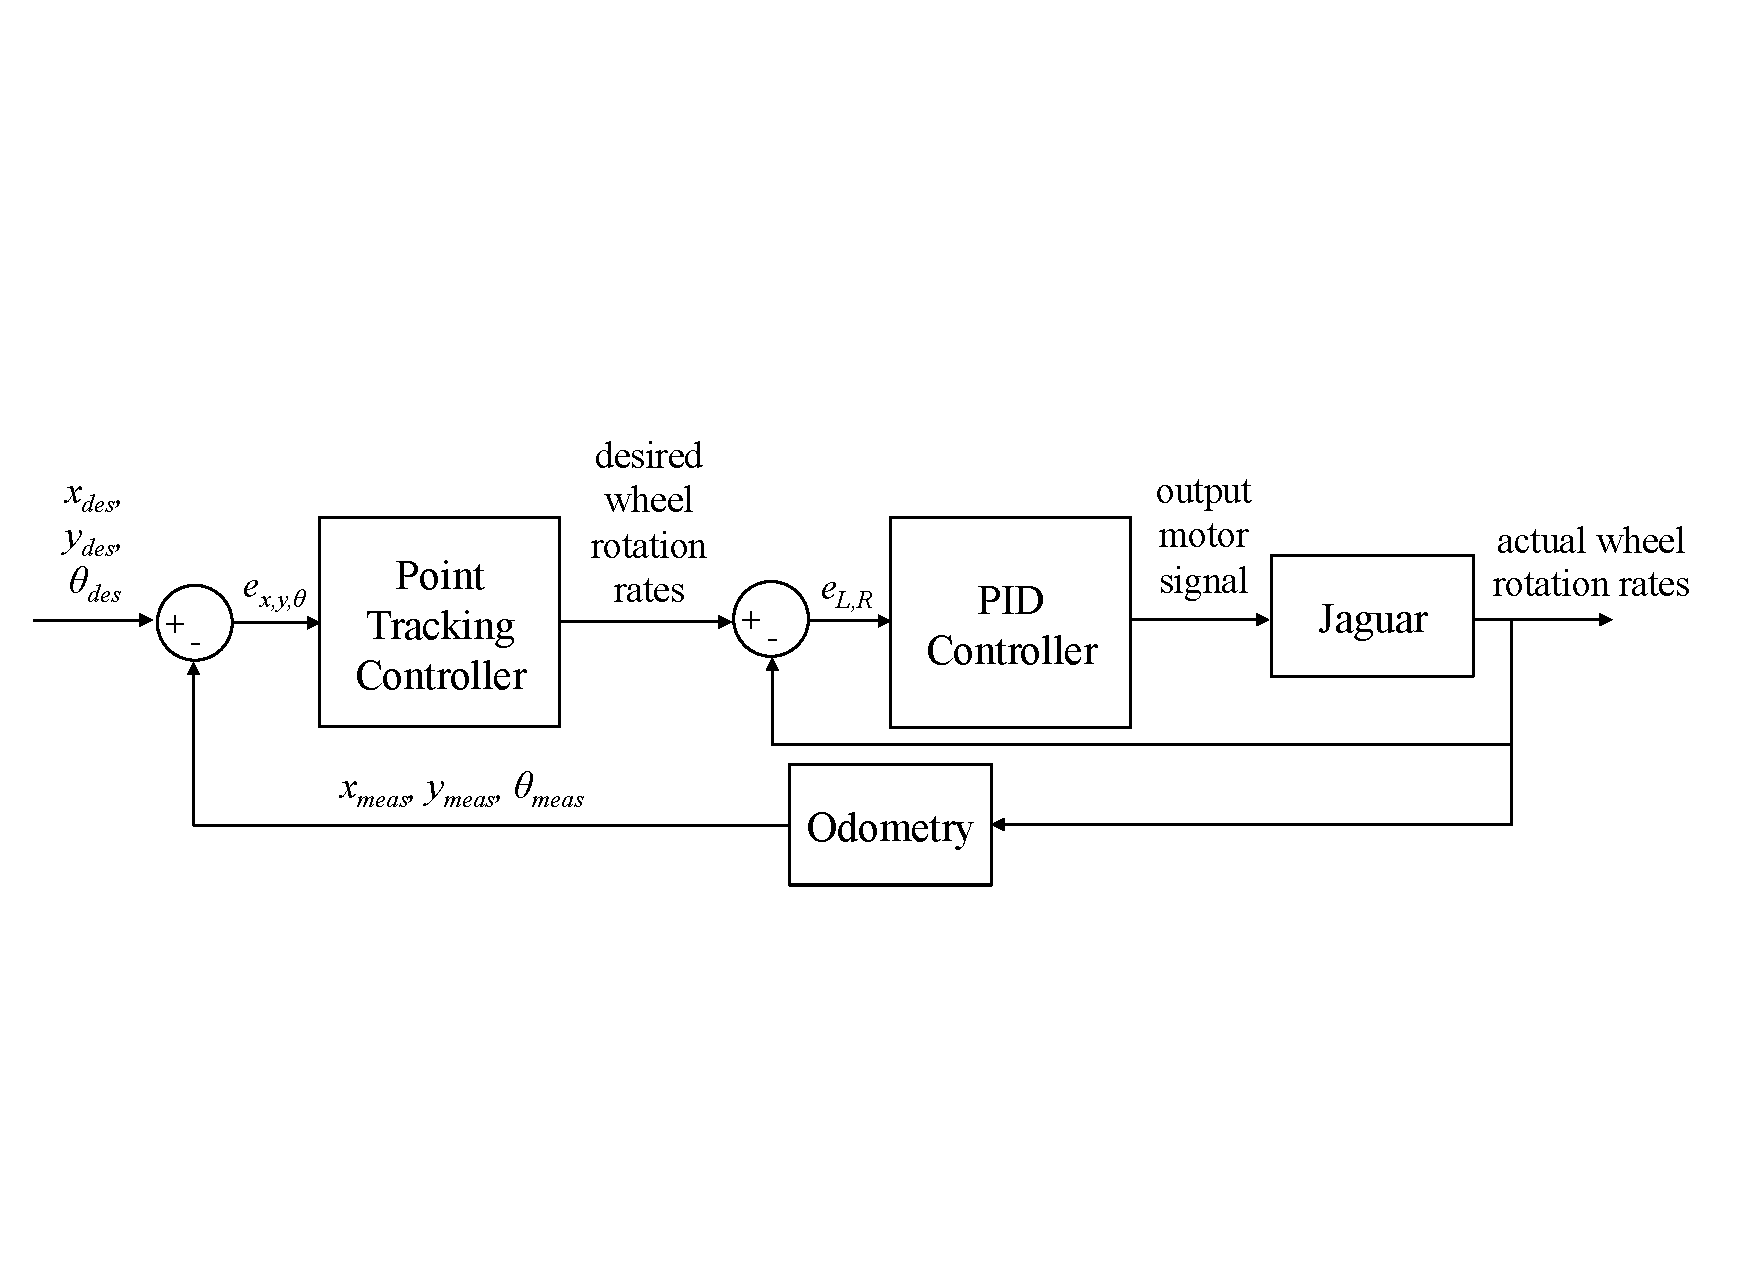
\includegraphics[width = 7cm]{figures/controlDiagram.pdf}
  \label{fig:control}}
  \subfigure[]{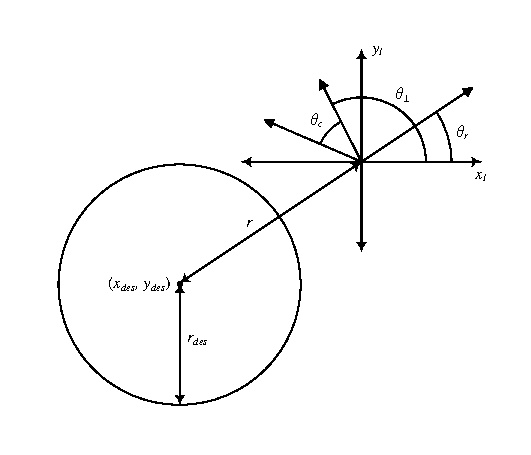
\includegraphics[width = 4.9cm]{figures/circle_controller.pdf}
  \label{fig:circle_con}}
  \subfigure[]{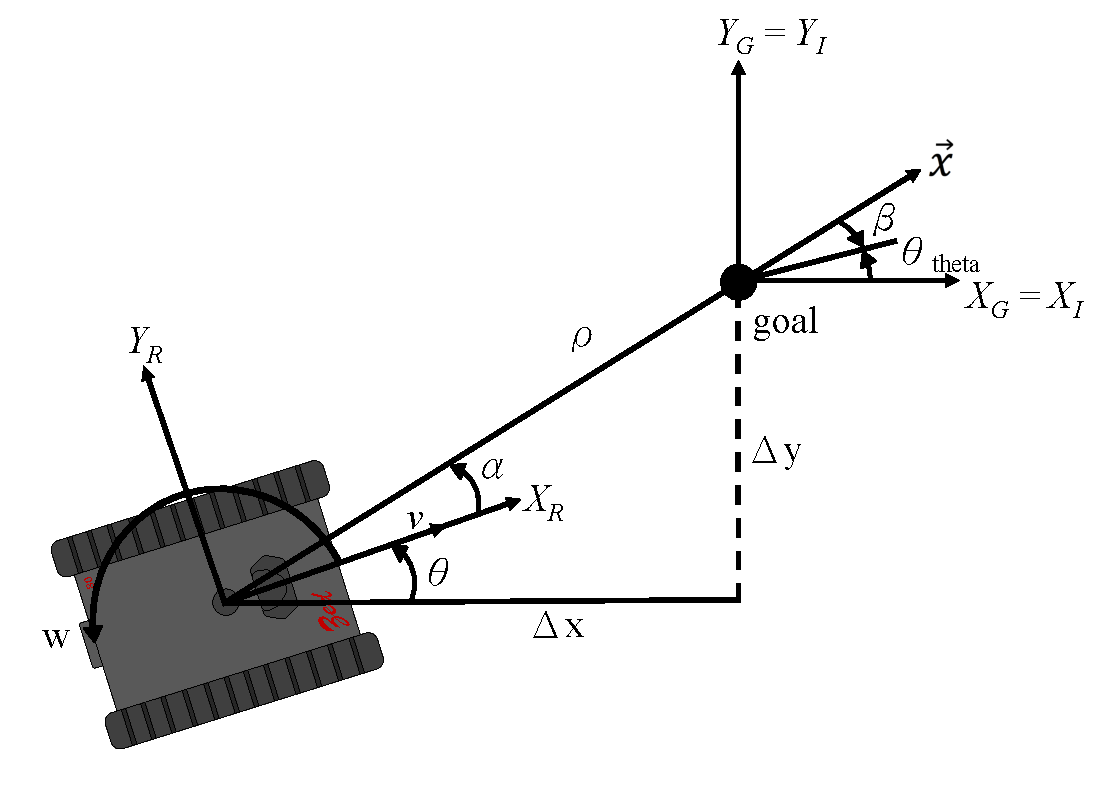
\includegraphics[width = 4.9cm]{figures/PointTracking.pdf}
  \label{fig:pttrack}}
  \caption{A block diagram of the overall Jaguar control system is shown in
           Fig.~\ref{fig:control}. An Overview of the circle tracking problem is
           shown in Fig.~\ref{fig:circle_con}.
           The position of the robot
           is given by the origin of the local coordinate frame $(x_l, y_l)$, and
           the desired circle is define by $(x_{des}, y_{des})$ and $r_{des}$. An overview of 
           the point tracking problem is shown in Fig.~\ref{fig:pttrack}.}
  \label{fig:controllers}
\end{figure*}


A control system was developed to move the Jaguar from its current position to its goal
position. Variables used are defined in Table~\ref{table:ptTrackVar}.

\begin{table}[htb]
  \resizebox{\columnwidth}{!}{
  \begin{tabular}{|c|l|}
    \hline
    Variable & Definition\\
    \hline
    $\alpha$ & angle between current and $\rho$ bearing\\
    $\beta$ & angle to get robot to desired bearing\\
    $w$ & rotational velocity of robot\\
	$\rho$ & distance between the current location and goal\\
    $\theta$ & angle of original bearing in $X_I-Y_I$ frame\\
    $\theta_{des}$ & desired end heading\\
    $\Delta x$ & $x$ distance between current and goal position in $X_I-Y_I$ frame\\
    $X_I,Y_I$& global coordinate frame\\
    $X_R,Y_R$& initial Jaguar reference frame\\
    $v$ & velocity of the Jaguar\\
    $\Delta y$ & $y$ distance between current and goal position in $X_I-Y_I$ frame\\
    \hline
  \end{tabular}
  }
  \label{table:ptTrackVar}
\end{table}
%
The three parameters, $\rho$, $\alpha$, and $\beta$ are defined in Eq.~\ref{eq:rho},
Eq.~\ref{eq:alpha}, and Eq.~\ref{eq:beta}, respectively.
\begin{align}
\rho &= \sqrt{\Delta x^2+\Delta y^2}
\label{eq:rho}\\
\alpha &= -\theta + \arctan 2(\Delta y, \Delta x)
\label{eq:alpha}\\
\beta &= -\theta - \alpha + \theta_{desired}
\label{eq:beta}
\end{align}
These equations assume the goal of the robot is in front of the robot, such that
$-\frac{\pi}{2} \leq \alpha \leq \frac{\pi}{2}$. For the case where the goal is behind the
robot, Eq.~\ref{eq:alpha} changes to Eq.~\ref{eq:alphaN}.
\begin{equation}
\alpha = -\theta + \arctan 2(-\Delta y, -\Delta x)
\label{eq:alphaN}
\end{equation}
For this control design, $\rho$, $\alpha$, and $\beta$, will be driven to zero to indicate
the Jaguar has reached the desired position. The control signals are the desired Jaguar
wheel rotation rates, which are set based on the desired robot velocity, $v$, and angular
velocity, $\omega$. The $v$ and $\omega$ are use the constants $K_{pho}$, $K_{alpha}$, and
$K_{beta}$ and can also be written in terms of the Jaguar's individual wheel angular
velocity, $\omega_1$ and $\omega_2$, as seen in Eq.~\ref{eq:v} and Eq.~\ref{eq:w}. $L$
describes the width of the Jaguar.
\begin{align}
v &= K_{\rho}*\rho = L*(\omega_1-\omega_2)
\label{eq:v}\\
w &= K_{\alpha}*\alpha+K_{\beta}*\beta = \omega_1+\omega_2
\label{eq:w}
\end{align}
In the case where the goal is behind the Jaguar, Eq.~\ref{eq:v} changes to Eq.~\ref{eq:vB}
\begin{equation}
v = -K_{\rho}*\rho
\label{eq:vB}
\end{equation}
These two variables describe the Jaguar's overall movement. For the point tracking system,
$v$ and $\omega$ are translated into the control input, which is the encoder pulses per
second of the wheel, using the previous two equations and Eq.~\ref{eq:om1} and
Eq.~\ref{eq:om2}. The left and right wheel velocities are $\psi_1$ and $\psi_2$,
respectively.
\begin{align}
\omega_1 &= \frac{r\dot{\psi}_1}{2L}
\label{eq:om1}\\
\omega_2 &= -\frac{r\dot{\psi}_2}{2L}
\label{eq:om2}
\end{align}
This gives the final equations Eq.~\ref{eq:psi1} and ~\ref{eq:psi2}, where $R$ is the
wheel radius.
\begin{align}
\psi_1 &= \frac{v + w L}{R}
\label{eq:psi1}\\
\psi_2 &= \frac{v - w L}{R}
\label{eq:psi2}
\end{align}
The final step to the control input involves converting $\psi_1$ and $\psi_2$ into the
desired wheel rotation rates, $\eta_{L,des}$ and $\eta_{R,des}$ using Eq.~\ref{eq:eta}.
\begin{equation}
\eta_{L,des;R,des}=\left(190\; \frac{pulses}{rotation}\right)\left(\frac{1\; rotation}{2\pi R\; meter}\right)\psi_{1,2}
\label{eq:eta}
\end{equation}

%%%%%%%%%%%%%%%%%%%%%%%%%%%%%%%%%%%%%%%%%
\subsection{Circle Tracking} \label{sec:circle_theo}
%%%%%%%%%%%%%%%%%%%%%%%%%%%%%%%%%%%%%%%%%

A non linear controller was developed to enable the robot to circle a desired point
$(x_{des}, y_{des})$ at a desired radius $r_{des}$.  An overview of the circle tracking
controller is shown in Fig.~\ref{fig:circle_con}.  Suppose that the robot is positioned at
the origin of the local coordinate frame $(x_l, y_l)$ shown in Fig.~\ref{fig:circle_con}.
The heading $\theta_{\perp}$ defines a vector that is tangent to line segment $r$. Observe
that $\theta_{\perp}$ would be the desired heading of the robot if $r$ = $r_{des}$.

The circle tracking controller sets a desired heading that is offset from $\theta_{\perp}$
by $\theta_{c}$ based on how far the robot is from the desired point, while setting a
constant speed of $v = \SI{0.25}{\m \s^{-1}}$. The circle tracking error is defined as
\begin{equation}
  \epsilon = |r| - |r_{des}|.
  \label{eq:err_circle}
\end{equation}
The offset angle at time $t$ given by
\begin{equation}
  \theta_c = \arctan(k\epsilon)
  \label{eq:theta_c}
\end{equation}
is then calculated based on $\epsilon$ determined using Eq.~\ref{eq:err_circle}, where $k$
is a constant.  Thus, if $\epsilon > 0$ in the case of the robot being too far from the
desired point, then $\theta_c$ will offset $\theta_{\perp}$ to drive the robot closer to
the center; the opposite happens if $\epsilon < 0$.  The desired heading is therefore
given by
\begin{equation}
  \theta_{des} = \theta_{\perp} + \theta_c.
  \label{eq:theta_des}
\end{equation}
Note that the circle tracking controller described is for a robot tracking a circle in the
counter-clockwise direction. Tracking in the clockwise direction can be done by negating
setting
\begin{equation}
  \theta_c = -\arctan(\epsilon).
\end{equation}

Since $\arctan$ has asymptotes at $\pi/2$ and $-\pi/2$, it follows that
Eq.~\ref{eq:theta_c} will never lead to a correction that causes the robot to travel away
from its desired point when it's too far or towards its desired point when it is too
close. The desired wheel speeds are then set according to Sec.~\ref{sec:circle_imp}.


%%%%%%%%%%%%%%%%%%%%%%%%%%%%%%%%%%%%%%%%%
\subsection{PID Controller} \label{sec:pid_theo}
%%%%%%%%%%%%%%%%%%%%%%%%%%%%%%%%%%%%%%%%%
The PID controller takes in the desired wheel rotation rates calculated in the point
tracking controller and sends the change in motor signal to the Jaguar. The controller
attempts to correct for the error (Eq.~\ref{eq:errorRotL} and ~\ref{eq:errorRotR}) between
the actual wheel rotation rates, $\eta_{L,act}$ and $\eta_{R,act}$, and the desired
rotation rates. 
\begin{align}
\epsilon_{L} &= \eta_{L,des}-\eta_{L,act}
\label{eq:errorRotL}\\
\epsilon_{R} &= \eta_{R,des}-\eta_{R,act}
\label{eq:errorRotR}
\end{align}
The controller uses the error, accumulation of error, and rate of error in the rotation
rate to calculate the motor signal.

%%%%%%%%%%%%%%%%%%%%%%%%%%%%%%%%%%%%%%%%%%%%%%%%%%%%%%%%%%%%%%%%%%%%%%%%%%%
\section{Control Implementation}\label{sec:implement}
%%%%%%%%%%%%%%%%%%%%%%%%%%%%%%%%%%%%%%%%%%%%%%%%%%%%%%%%%%%%%%%%%%%%%%%%%%%

%%%%%%%%%%%%%%%%%%%%%%%%%%%%%%%%%%%%%%%%%
\subsection{Point Tracking}
%%%%%%%%%%%%%%%%%%%%%%%%%%%%%%%%%%%%%%%%%

The structure of the point tracker, shown in Alg.~\ref{alg:ptTracker}, has two steps:
travel to point and rotate to point. If the Jaguar is not at its goal, given a certain
threshold, the function called is \textsc{travelToPoint()}. If the Jaguar is at its goal
but not at the correct heading, the function called is \textsc{rotateToPoint()}. At the
end, the desired rotation rate for the left and right wheels are checked against a
threshold; if smaller, the Jaguar is stopped because it has reached its desired goal with
the appropriate heading.

\begin{algorithm}[h]
  \caption{FlyToSetPoint() function}
  \begin{algorithmic}[1]
      \State $\Delta x \gets x_{des}-x_{meas}$
      \State $\Delta y \gets y_{des}-y_{meas}$
      \State $\text{distanceToTarget} \gets \sqrt{\Delta x^2+\Delta y^2}$
      \medskip
      \If{$\text{distanceToTarget} > \text{distanceToThreshold}$}
      \State $\textsc{travelToPoint}()$
      \Else
          \State $\textsc{rotateToPoint}()$
      \EndIf
      \medskip

    \end{algorithmic}
  \label{alg:ptTracker}
\end{algorithm}

The \textsc{travelToPoint()} function calculates the angle between the current heading and
direction heading, which is the heading for the shortest path. This angle was used to
determine if the goal position was in front of or behind the Jaguar. Eq.~\ref{eq:rho},
~\ref{eq:alpha}, ~\ref{eq:beta}, and ~\ref{eq:alphaN} were used to calculate $\rho$,
$\alpha$, and $\beta$. Based on these values, the desired Jaguar $v$ and $w$ were
calculated using Eq.~\ref{eq:v} and ~\ref{eq:w}. Finally, the velocities $\psi_1$ and
$\psi_2$ were calculated using Eq.~\ref{eq:psi1} and ~\ref{eq:psi2} and converted to
$\nu_{L,des}$ and $\nu_{R,des}$. The wheel velocities was capped using a scaling ratio
between the two wheels to allow the feedback loop enough time to respond to the system.

%%%%%%%%%%%%%%%%%%%%%%%%%%%%%%%%%%%%%%%%%
\subsection{Circle Tracking} \label{sec:circle_imp}
%%%%%%%%%%%%%%%%%%%%%%%%%%%%%%%%%%%%%%%%%

The implementation of the circle tracking controller on hardware uses
Eq.~\ref{eq:err_circle}, Eq.~\ref{eq:theta_c}, and Eq.~\ref{eq:theta_des} to calculate a
desired heading $\theta_{des}$. A value of $k = 1$ was chosen empirically for
Eq.~\ref{eq:theta_c}. The robot's desired rotational speed $w$ proportional to the
difference between the robot's actual heading and its desired. Recall from
section~\ref{sec:circle_theo} that the circle controller sets a constant speed $v$.  The
equations Eq.~\ref{eq:psi1} and Eq.~\ref{eq:psi2} are then used to determine the desired
wheel rotation speeds using $w$ and $v$.

%%%%%%%%%%%%%%%%%%%%%%%%%%%%%%%%%%%%%%%%%
\subsection{Wheel Speed Control} \label{sec:pid_imp}
%%%%%%%%%%%%%%%%%%%%%%%%%%%%%%%%%%%%%%%%%
The wheel speed is calculated using a PID controller, as seen in Alg.~\ref{alg:PID}.
Eq.~\ref{eq:errorRotL} and Eq.~\ref{eq:errorRotR} are used to calculate the rotation rate
error, $\epsilon_L$ and $\epsilon_R$, which are used in the P term of the controller. The
integral term involves accumulating the error over time, which is implemented in
Alg.~\ref{alg:PID}, line 1. The $0.9$ constant in $\epsilon_{sumL}$ and $\epsilon_{sumR}$
scales down how much error is accumulating over time, which helps to minimize the chance
of the error from blowing up. The derivative term involves the change in rate of error
over time, implemented in Alg.~\ref{alg:PID}, line 2. In the actual code, a moving average
filter is applied to the $dErr_L$ and $dErr_R$ variables to smooth out the effect of the D
term in the control.

\begin{algorithm}[h]
  \caption{CalcMotorSignals() function}
  \begin{algorithmic}[1]
  \State $K_P \gets 2.5$
  \State $K_D \gets 0.1$
  \State $K_I \gets 0.0$
  \medskip
  \State $\epsilon_{sumL,sumR} \gets 0.9\; \epsilon_{sumL,sumR}+\epsilon_{L,R} \Delta t$
  \State $dErr_{L,R} \gets (\epsilon_{L,R}-\epsilon_{lastL,lastR}) / \Delta t$
  \State $u_{L,R}=K_P*\epsilon_{L,R} + K_I*\epsilon_{sumL,sumR} + K_D*dErr_{L,R}$
  \State $accum_{L,R}=accum_{L,R}+u_{L,R}$
  \medskip
  \If{$\eta_{Ldes,Rdes} \gets 0$}
  \State $\text{motorSignal}_{L,R} \gets \text{zeroOutput}$
  \Else
  \State $\text{motorSignal}_{L,R} \gets \text{zeroOutput} \pm \text{deadBand}$ 
  \Statex \hspace{4.8cm} $ \pm accum_{L,R}$
	\EndIf
    \end{algorithmic}
  \label{alg:PID}
\end{algorithm}

The control signals, which are the changes in the wheel rotation rates $u_L$ and $u_R$,
are calculated in Alg.~\ref{alg:PID}, line 5-8. Two factors were considered in the
hardware implementation: the deadband and the control signal output. The deadband is a
range where a physical system cannot perform what the control signal specifies. The
problem is that the $K_P$ value in the PID control needs to be increased to overcome this
range. However, the larger $K_P$ value negatively affects the Jaguar after the range is
passed; the larger value causes a larger response to the error, resulting in overshoot. To
account for this problem, line 8 in Alg.~\ref{alg:PID} shows the offset the output motor
signal called deadBand. This way the Jaguar either jumps from a zero motor signal to one
offset by the deadBand constant that takes the robot out of the deadband range.

Another hardware factor is the output from the PID controller to the Jaguar. Based on
Alg.~\ref{alg:PID}, the control signals $u_L$ and $u_R$ are the necessary changes in the
wheel rotation rates. Since motorSignal$_{L}$ and motorSignal$_{R}$ are offset by both
zeroOutput and deadBand, the algorithm requires a to keep track of how the wheel rotation
rates change over time. Thus, the $accum_L$ and $accum_R$ accumulate those changes over
time to ensure the new control signal is added to the previous one.

\begin{figure*}[t]
  \centering
  \subfigure[]{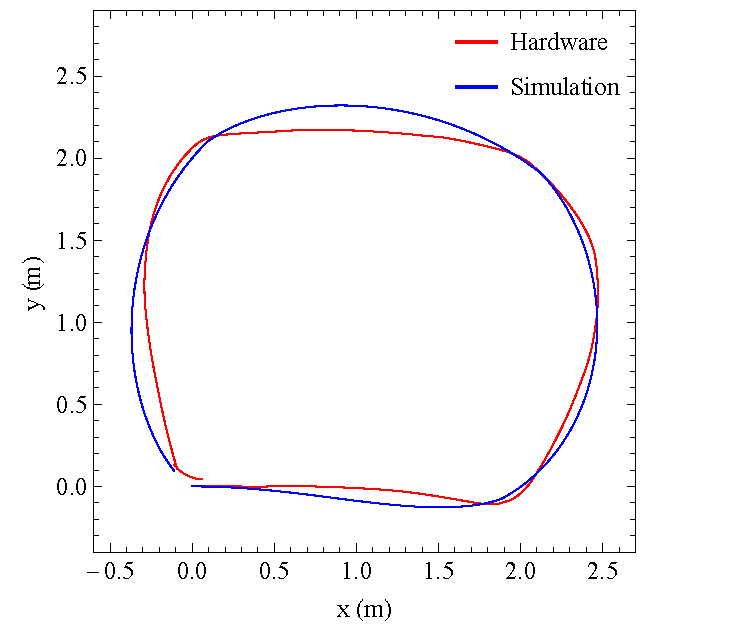
\includegraphics[width = 5.6cm]{figures/square.pdf}
  \label{fig:squareTraj}}
  \subfigure[]{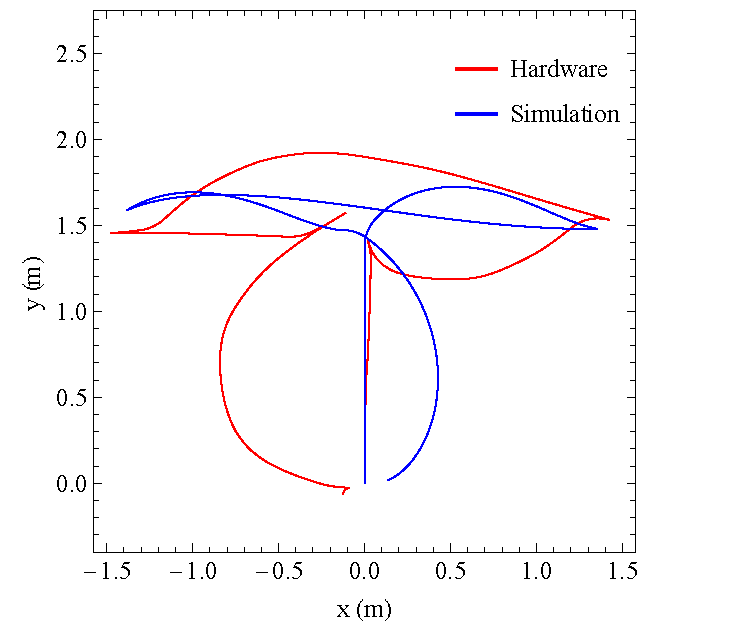
\includegraphics[width = 5.6cm]{figures/t_shape.pdf}
  \label{fig:tTraj}}
  \subfigure[]{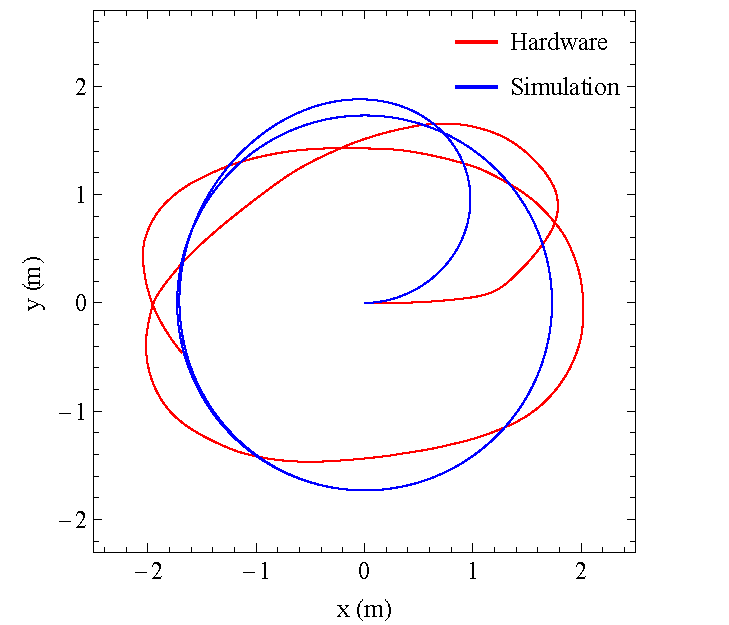
\includegraphics[width = 5.6cm]{figures/circle.pdf}
  \label{fig:circTraj}}
  \caption{Trajectory plots from hardware and simulation tests are shown. A square, T-shape, and circle trajectory are used to demonstrate the controller performance.}
  \label{fig:trajectories}
\end{figure*}


\begin{figure*}[t]
\centering
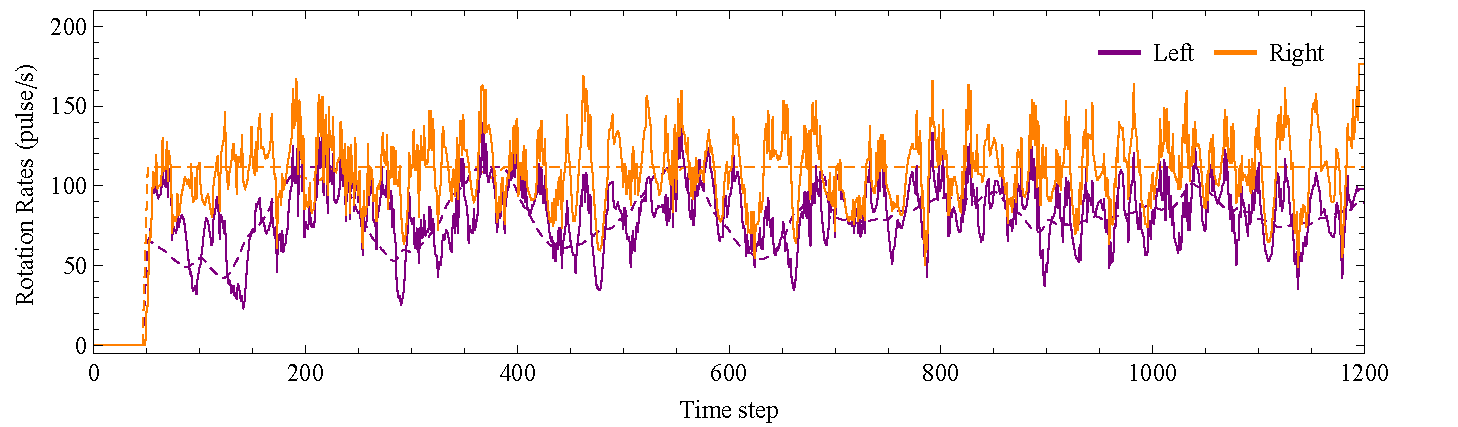
\includegraphics[width=18cm]{figures/pid_err.pdf}
\caption{Comparison of actual and desired wheel rotation speeds. The desired rotation
         speeds are shown by the dotted lines and the actual rotation speeds are
         shown by the solid lines.}
\label{fig:pid_err}
\end{figure*}

%%%%%%%%%%%%%%%%%%%%%%%%%%%%%%%%%%%%%%%%%%%%%%%%%%%%%%%%%%%%%%%%%%%%%%%%%%%
\section{Results and Discussions}
%%%%%%%%%%%%%%%%%%%%%%%%%%%%%%%%%%%%%%%%%%%%%%%%%%%%%%%%%%%%%%%%%%%%%%%%%%%

Experiments were conducted in both simulation and hardware to verify the controllers
described in the previous section. The results followed by discussion are presented in the
following subsections.

%%%%%%%%%%%%%%%%%%%%%%%%%%%%%%%%%%%%%%%%%
\subsection{Trajectories}
%%%%%%%%%%%%%%%%%%%%%%%%%%%%%%%%%%%%%%%%%
Three tests were performed to capture behavior of the robot driving in straight lines,
making turns, navigating to points behind itself, and driving in a circle. The results are
shown in Fig.~\ref{fig:trajectories}. In Fig.~\ref{fig:squareTraj}, a trajectory of a
\SI{2}{m} square was used starting from the origin and moving counterclockwise. For the
T-shape trajectory in Fig.~\ref{fig:tTraj}, the Jaguar starts at the origin and creates a
\SI{1.5}{m} stem and a \SI{3}{m} hat. The circle trajectory, Fig.~\ref{fig:circTraj}, has
a radius of \SI{1.5}{m} and also starts at the origin.

%%%%%%%%%%%%%%%%%%%%%%%%%%%%%%%%%%%%%%%%%
\subsection{Simulation and Hardware Performance}
%%%%%%%%%%%%%%%%%%%%%%%%%%%%%%%%%%%%%%%%%
Both the simulated and hardware trajectories from Fig.~\ref{fig:squareTraj} and
~\ref{fig:tTraj} reach the specified positions and orientations within the set threshold.
However, there are differences in the paths taken, which is may be based on the
theoretical model used in the simulation.

In Fig.~\ref{fig:squareTraj}, the Jaguar makes sharper turns around the corner than the
simulated trajectory. There are a many factors that could be cause this to happen, such as
PID tuning (discussed in Sec.~\ref{sec:PIDtune}) or discrepancies between the theoretical
model and physical system. The hardware trajectory was left of the simulation trajectory
(relative to the Jaguar's reference frame) for three of the four square sides. This may be
from motor response to input signals or varying deadband ranges between wheels.

In the T-shape trajectories seen in Fig.~\ref{fig:tTraj}, the Jaguar takes a wider path in
hardware than in simulation. Tracing the path at set point $(0,1.5)$, the simulation moves
forward to $(1.5,1.5)$, while the actual Jaguar moves backward to the same point. Even
though the heading at $(1.5,1.5)$ is set to zero, the Jaguar likely hits the desired
position and begins moving to the next point without time to correct for the heading.
Because of the different paths taken from $(0,0)$ to $(0,1.5)$, the Jaguar could have been
at a heading that considered the set point $(1.5, 1.5)$ to be behind the robot, whereas in
the simulation, the robot found the point to be in front of it. Moreover, more tuning in
the PID constants may also minimize the discrepancies.

Variation between the circle trajectories in hardware and simulation shown in
Fig.~\ref{fig:circTraj} is discussed in Sec.~\ref{sec:circT}.

\addtolength{\textheight}{-13.4cm}

%%%%%%%%%%%%%%%%%%%%%%%%%%%%%%%%%%%%%%%%%
\subsection{Wheel Velocity PID Performance} \label{sec:PIDtune}
%%%%%%%%%%%%%%%%%%%%%%%%%%%%%%%%%%%%%%%%%

A comparison of the actual and desired wheel rotation speeds set by the PID wheel speed
controller is shown in Fig.~\ref{fig:pid_err}.  The desired wheel rotation speeds
correspond to the circular trajectory performed on hardware shown in
Fig.~\ref{fig:circTraj}.  It can be seen from Fig.~\ref{fig:pid_err} that the desired
rotation rates oscillates around the set points.

The response could be smoothed by decreasing the proportional gain and by increasing the
derivative gain term, which is currently set two order of magnitudes lower than the
proportional gain.

Another possible reason for the oscillation observed in the response could be due to the
limited resolution of the encoders. Since the actual rotation rate could be as low as 50
pulses per second and the control loop runs at \SI{10}{\Hz}, there is limited resolution
in the difference in encoder readings. This implies that setting the control rate too high
could exacerbate the resolution issue and make stability even worse.

\begin{figure}[t]
\centering
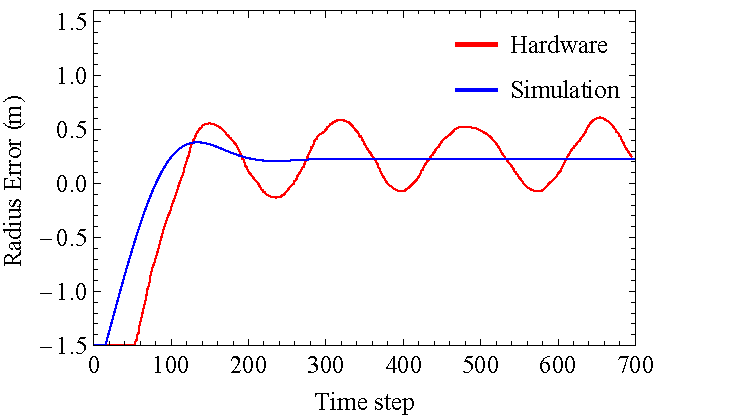
\includegraphics[width=3in]{figures/circle_err.pdf}
\caption{Difference between the desired radius and actual distance to circle origin
         of the circular trajectories presented in Fig.~\ref{fig:circTraj}}.
\label{fig:circle_err}
\end{figure}

%%%%%%%%%%%%%%%%%%%%%%%%%%%%%%%%%%%%%%%%%
\subsection{Circle Tracking Error}\label{sec:circT}
%%%%%%%%%%%%%%%%%%%%%%%%%%%%%%%%%%%%%%%%%

The tracking error of the circular trajectory shown in Fig.~\ref{fig:circTraj} is shown in
Fig.~\ref{fig:circle_err}. Here, tracking error is defined as the difference between
actual distance from circle origin and desired circle radius.  For the simulation, it can
be seen that tracking error stabilizes after 250 time steps.  However, tracking error
oscillates in hardware tests. This suggests that the constant $k$ in Eq.~\ref{eq:theta_c}
can be lowered to decrease the response and dampen the oscillations.

The steady state error of approximately \SI{0.25}{\meter} in simulation can be explained
as follows. Suppose that the robot is at the point on the circle that intersects $r_{des}$
in Fig.~\ref{fig:circle_con} and has a heading tangent to $r_{des}$.  Based on
Eq.~\ref{eq:theta_c}, the desired heading will be the same as the robot's current heading.
It follows that the distance of the robot to the circle origin will be greater than the
desired radius at the next time step. Therefore, the circle tracking controller described
in Sec.~\ref{sec:circle_imp} will have a steady state error that decreases with the update
rate of the control loop. This steady state error can be corrected by introducing an
integral term in the circle tracking controller.

%%%%%%%%%%%%%%%%%%%%%%%%%%%%%%%%%%%%%%%%%%%%%%%%%%%%%%%%%%%%%%%%%%%%%%%%%%%
\section{Conclusion}
In this paper, the closed-loop controller was shown to drive the Jaguar to its desired
state in both simulation hardware. The Jaguar can also follow a specified trajectory,
although its paths differ from the theoretical model's. For the points in the trajectory,
the Jaguar did not always reach the correct bearing. This difference in path and bearing
may come from the PID constants and hardware issues, such as encoder resolution and motor
deadbands. To correct for these mistakes and create a stable system, the PID constants can
be better tuned.
%%%%%%%%%%%%%%%%%%%%%%%%%%%%%%%%%%%%%%%%%%%%%%%%%%%%%%%%%%%%%%%%%%%%%%%%%%%

\nocite{*}
\bibliographystyle{ieeetran}
\bibliography{citations}

\end{document}
